\documentclass[a5paper,titlepage,10pt,openany]{scrbook}
\usepackage[a5paper,backref]{hyperref}
\usepackage[papersize={148.5mm,215mm},twoside,bindingoffset=0.5cm,hmargin={2cm,2cm},
				vmargin={2cm,2cm},footskip=1.1cm,driver=dvipdfm]{geometry}
\usepackage{palatino}
\usepackage{pstricks}
\usepackage{graphicx}
\usepackage[bahasa]{babel} 
%\usepackage[pdftex]{dropping}
\usepackage{lettrine}
\usepackage{pifont}
\usepackage{enumitem}
\usepackage{wrapfig}
\usepackage{indentfirst}

\author{Lingkungan St. Petrus Maguwo}
\title{Warta Iman}
\setlength{\parindent}{1cm}
\psset{unit=1mm}

\makeatletter
\renewcommand{\@makeschapterhead}[1]{%
  {\parindent \z@ \centering \normalfont
    \interlinepenalty\@M \Large \bfseries #1\par\nobreak \vskip 20\p@ }}
\renewcommand{\section}{\@startsection {section}{1}{\z@}%
                                   {-3.5ex \@plus -1ex \@minus -.2ex}%
                                   {2.3ex \@plus.2ex}%
%                                   {\normalfont\normalsize\bfseries\centering}}
                                   {\normalfont\normalsize\bfseries}}
\renewcommand\subsection{\@startsection{subsection}{2}{\z@}%
                                     {-3.25ex\@plus -1ex \@minus -.2ex}%
                                     {1.5ex \@plus .2ex}%
                                     {\normalfont\normalsize\bfseries}}
\renewcommand\subsubsection{\@startsection{subsubsection}{3}{\parindent}%
                                    {3.25ex \@plus1ex \@minus.2ex}%
                                    {-1em}%
                                    {\normalfont\normalsize\bfseries}}

\makeatother

\makeatletter  % Allow the use of @ in command names
\long\def\@makecaption#1#2{%
  \vskip\abovecaptionskip
  \sbox\@tempboxa{{#1#2}}%
  \ifdim \wd\@tempboxa >\hsize
    {#1#2\par}
  \else
    \hbox to\hsize{\hfil\box\@tempboxa\hfil}%
  \fi
  \vskip\belowcaptionskip}
\makeatother   % Cancel the effect of \makeatletter

\newcommand{\chap}[1]{%
    \chapter*{#1}
	\addcontentsline{toc}{chapter}{#1}
    }

\newcommand{\sumber}[1]{%    
	\begin{flushright}
	{\emph{#1}}
	\end{flushright}
}
\hyphenation{sa-u-da-ra-ku}
\hyphenation{ke-ri-ngat}
\hyphenation{je-ri-tan}
\hyphenation{hu-bung-an}
\hyphenation{me-nya-dari}
\hyphenation{Eng-kau}
\hyphenation{ke-sa-lah-an}
\hyphenation{ba-gai-ma-na}
\hyphenation{Tu-han}
\hyphenation{di-per-ca-ya-kan}
\hyphenation{men-ja-uh-kan}
\hyphenation{bu-kan-lah}
\hyphenation{per-sa-tu-kan-lah}
\hyphenation{ma-khluk}
\hyphenation{Sem-buh-kan-lah}
\hyphenation{ja-lan}
\hyphenation{mem-bu-tuh-kan}
\hyphenation{be-ri-kan-lah}
\hyphenation{me-ra-sa-kan}
\hyphenation{te-man-ilah}
\hyphenation{mem-bi-ngung-kan}
\hyphenation{di-ka-gum-i}
\hyphenation{ta-ngis-an-Mu}
\hyphenation{mi-lik-ilah}

\renewcommand{\figurename}{~}
\renewcommand\thefigure{~}

\begin{document}
\pagestyle{plain}
\thispagestyle{empty}
\newcommand{\edisi}[1]{%
\DeclareFixedFont{\PT}{T1}{ppl}{b}{}{0.7in}
\DeclareFixedFont{\PTit}{T1}{ppl}{b}{it}{0.7in}
\DeclareFixedFont{\PTsmall}{T1}{ppl}{b}{it}{0.25in}
\DeclareFixedFont{\PTsmaller}{T1}{ppl}{b}{it}{0.175in}
\DeclareFixedFont{\PTsmallest}{T1}{ppl}{b}{it}{0.15in}

\begin{pspicture}(14cm,2cm)
\rput[rb](10.35cm,3cm){\PTsmallest {#1}}
\rput[lb](-2cm,1.5cm){\PT {WARTA IMAN}}
\rput[lb](0cm,0.5cm){\PTsmall {Lingkungan St. Petrus Maguwo}}
\end{pspicture}%
}

\newcounter{kgkcounter}[chapter]
\renewcommand{\thekgkcounter}{\arabic{kgkcounter}. }
\newcommand{\kgk}[1]{\refstepcounter{kgkcounter}\textbf{\flushleft \textbf{\thekgkcounter #1}}\\}

\newcommand{\kutipan}[1]{%
\noindent{\framebox{\parbox{10cm}{\centering\emph{#1}}}}}

\edisi{November 2011}

%\vspace{1cm}

\begin{center}
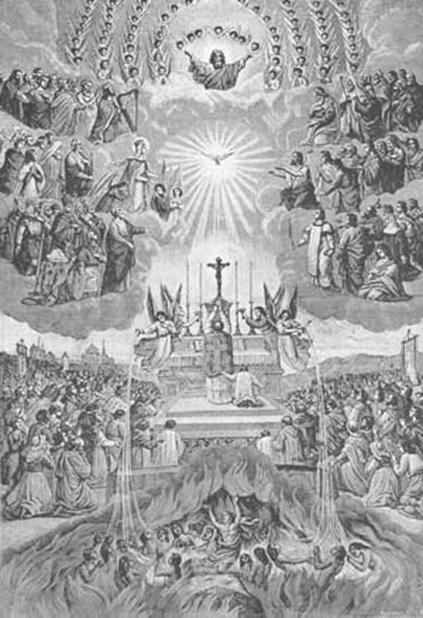
\includegraphics[scale=0.85]{gambar/purgatory2.jpg}
\end{center}

%\vspace{1cm}

\begin{center}
{\PTsmaller {Kasih, kerendahan hati, dan menurut pada kehendak Allah }}
\end{center}

\newpage

\chapter*{Dari Redaksi}
\footnotesize
\indent{Berkah Dalem,}
Bulan Maret sudah memasuki masa Prapaskah. Tidak ada salahnya jika kita mengambil tema \textit{Prapaskah} untuk edisi kali ini. Mungkin kita masih bertanya-tanya kenapa setiap masa prapaskah kita berpuasa dan berpantang. Bagian awal WI edisi kali mencoba menjawab pertanyaan tersebut.

\bigskip
Menjelang prapaskah kita sudah mendengar pembacaan pesan Bapa Uskup dalam menyongsong masa prapaskah. Dalam edisi ini Anda dapat menyimak pesan dari Bapa Paus Benediktus dalam rangka menyongsong Prapaskah 2012.

\bigskip
Masa prapaskah diawali dengan hari Rabu Abu. Kenapa Rabu dan kenapa abu? Juga kenapa digunakan daun palm bukan yang lain? Jawabannya dapat Anda simak dalam edisi kali ini. 
 
\bigskip
Renungan tentang 4 prinsip hidup dan ketika garam kehilangan asinnya melengkapi edisi kali ini. Kutipan Kompendium Gereja Katolik masih berlanjut sampai pada nomor 30 -- 33.

\bigskip

Warta lingkungan kali ini tidak memuat pasangan yang berulangtahun, karena data yang ada redaksi tidak ditemukan warga St. Petrus yang berulangtahun perkawinan bulan Maret. Redaksi tetap berharap partisipasi umat untuk meramaikan rubrik ini dengan mengirim sms berupa saran, kritik, pertanyaan, atau sekedar \textit{uneg-uneg}, dengan harapan terjalin komunikasi antar umat dan juga pengurus. Tema bulan April adalah Paskah sedang bulan Mei adalah Liturgi. Sekali lagi ditunggu partisipasi seluruh umat.
\normalsize

\begin{center}***\end{center} 

\vfill

\noindent{\framebox{\parbox{10cm}{\small
Warta Iman\\
Media komunikasi dan informasi umat lingkungan St. Petrus\\
Alamat Redaksi: Lingkungan St. Petrus Maguwo\\
E-mail: stpetrusmgw@gmail.com
}}}
\normalsize


\tableofcontents
\chap{Kebangkitan Badan}

Kehidupan manusia di dunia ini berakhir dengan kematian. Pada saat kematian, tubuh manusia mengalami kehancuran sedangkan jiwanya melangkah menuju Allah dan emnunggu saat disatukan kembali dengan tubuh baru. Kebangkitan badan adalah kebangkitan orang-orang benar dari mati dalam tubuh yang baru, sebagai kebangkitan definitif untuk kehidupan abadi. Dengan bangkit dari mati, orang-orang benar akan mengalami eksistensinya yang baru. Sesudah kematian, tidak hanya jiwa kita yang hidup terus tetapi ``tubuh kita yang fana'' ini juga akan hidup kembali dalam kondisi yang samasekali baru (KGK 990)

Ajaran iman Katolik mengatakan bahwa setelah kematian ada kebangkitan badan dan kehidupan kekal.
Pada saat orang meninggal dunia, maka badan/tubuhnya akan terpisah dengan jiwanya. Badan yang dikubur/dikremasi – kembali menjadi debu, dan jiwa/rohnya akan kembali pada Allah. Dihadapan Allah, jiwa orang itu akan diadili (pengadilan khusus) berdasar perbuatan dan imannya untuk menentukan nasib selanjutnya.
\begin{itemize}
\item Jika perbuatan dan imannya tanpa cela, maka upahnya adalah langsung masuk surga
\item Jika berimankan Allah, pekerjaan baik, namun kadang masih jatuh dalam dosa --bertobat-dosa lagi-- bertobat lagi, maka mereka akan ditempatkan sementara dalam api penyucian untuk dimurnikan dosa-dosanya. Jika saatnya tiba, atas belas kasih Allah dan doa-doa serta kurban dari umat yang masih hidup, maka mereka juga akan masuk surga.
\item Jika imannya menentang Allah, secara sadar dan tanpa paksaan melakukan perbuatan yang sangat jahat dan tidak bertobat, maka nerakalah upahnya.
\end{itemize}

Pada akhir zaman, pada waktu kedatangan Kristus yang kedua kalinya, akan terjadi kebangkitan badan
Pada saat Kebangkitan badan, Kristus akan membangkitkan kembali tubuh semua orang yang sudah meninggal, namun dengan tubuh baru dan menyatukannya kembali dengan jiwa/roh masing-masing. Kita tidak tahu persisnya kapan, namun secara definitif hal itu terjadi pada hari kiamat atau akhir zaman. Meskipun demikian, di pihak lain, kita sebenarnya telah bangkit bersama Kristus dalam arti tertentu. Oleh Roh Kudus, kehidupan Kristen di dunia ini sudah merupakan keikutsertaan pada kematian dan kebangkitan Kristus:

\begin{quote}
\textit{Karena dengan Dia kamu dikuburkan dalam baptisan, dan di dalam Dia kamu turut dibangkitkan juga oleh kepercayaanmu kepada kerja kuasa Allah, yang telah membangkitkan Dia dari orang mati. \ldots
Karena itu, kalau kamu dibangkitkan bersama dengan Kristus, carilah perkara yang di atas, di mana Kristus ada, duduk di sebelah kanan Allah.
}(Kol 2:12; 3:1)
\end{quote}   

\noindent{Dari surat St. Paulus kepada jemaat di Korintus tertulis, }

\begin{quote}
\textit{Tetapi mungkin ada orang yang bertanya: 'Bagaimanakah orang mati dibangkitkan? Dan dengan tubuh apakah mereka akan datang kembali?' Hai orang bodoh! Apa yang engkau sendiri taburkan, tidak akan tumbuh dan hidup, kalau ia tidak mati dahulu. Demikianlah pula halnya dengan kebangkitan orang mati. Ditaburkan dalam kebinasaan, dibangkitkan dalam ketidakbinasaan. Ditaburkan dalam kehinaan, dibangkitkan dalam kemuliaan. Ditaburkan dalam kelemahan, dibangkitkan dalam kekuatan. Yang ditaburkan adalah tubuh alamiah, yang dibangkitkan adalah tubuh rohaniah.} (1 Kor 15:35-36, 42-44).
\end{quote}

Tubuh kaum beriman akan diubah serupa dengan Tubuh Kristus yang bangkit. Menurut teologi, tubuh yang mulia dan sempurna ini memiliki karakteristik: identitas, keutuhan dan keabadian, dengan empat ``kualitas transenden''
\begin{enumerate} 
\item ``\textbf{tak dapat rusak}'', atau bebas dari kerusakan fisik, kematian, penyakit, dan rasa sakit; 
\item ``\textbf{semarak}'' atau bebas dari cacat dan dikaruniai keindahan dan cahaya; 
\item ``\textbf{leluasa}'' di mana jiwa menggerakkan tubuh dan adanya kebebasan gerak; 
\item ``\textbf{halus}'', di mana tubuh sepenuhnya dirohanikan di bawah kuasa jiwa. Katekismus mengajarkan, ``Sesudah pengadilan umum, semua orang yang benar, yang dimuliakan dengan jiwa dan badannya, akan memerintah bersama Kristus sampai selama-lamanya.'' (KGK no. 1042).
\end{enumerate}

Bagi tubuh dari jiwa-jiwa yang dikutuk di neraka
walaupun mereka akan memiliki identitas, keutuhan dan keabadian, tetapi tidak memiliki keempat kualitas transenden. Mereka memiliki kondisi yang memungkinkan mereka menderita hukuman abadi di neraka, tetapi tidak memiliki kemuliaan Kristus yang dikaruniakan bagi mereka yang ada di surga.

Pada saat kedatangan Kristus yang kedua kalinya, akan terjadi pengadilan terakhir. Tidak ada yang tahu kapan saat itu terjadi. Hanya Bapa yang tahu kapan dan bagaimana semua akan berlangsung. Allah Bapa melalui PutraNya Yesus Kristus akan membuat penilaian ata seluruh sejarah kehidupan manusia dan ciptaanNya. Pengadilan terakhir akan membuktikan keadilan Allah yang mengatasi segala ketidakadilan seluruh makhluk ciptaanNya dan akan membuktikan bahwa cintaNya lebih besar daripada kematian (KGK 1040)

Tidak ada yang tersembunyi di mata Allah, dan di hadapan Kristus sebagai hakim, semuanya akan dibuka dan akan terlihat nyata hubungan setiap manusia dengan Allah yang sebenarnya. Pengadilan terakhir akan membuka sampai ke akibat-akibat yang paling jauh, kebaikan apa yang dilakukan atau tidak dilakukan oleh setiap orang selama hidup di dunia ini. (KGK 1039)

Kepercayaan mengenai adanya pengadilan terakhir mengajak semua orang agar bertobat. Selain itu, kita juga diingatkan bahwa kehidupan di dunia ini adalah kesempatan penuh rahmat untuk melakukan pertobatan. Tidak ada orang yang tahu kapan kita mati dan juga tidak ada yang tahu kapan akhir zaman tiba. Ajaran tentang pengadilan terakhir mengajak orang untuk membangun pertobatan sejak sekarang, sebelum semuanya terlambat. Adanya pengadilan terakhir dapat saja menimbulkan ketakutan akan Allah, namun dapat saja menjadi kerinduan dari orang-orang benar dan saleh. Semua orang benar akan memperoleh apa yang selama ini dirindukannya, yaitu saat persatuan dengan Allah dalam kehidupan abadi. Bagi orang benar, saat itu menjadi saat rahmat yang akan membuat orang merasakan kebahagiaan karena diperkenankan bersatu dengan Allah Tritunggal dan para kudus dalam kehidupan abadi.
\sumber{PAS}
\small

\chap{Rahasia Arwah-arwah di Api Penyucian}
\begin{center}\large
Wawancara dengan Maria Simma dari Austria
\normalsize
\end{center}
\setlength{\parindent}{0cm}
\renewcommand{\figurename}{~}

\begin{wrapfigure}{l}{3cm}
\centering
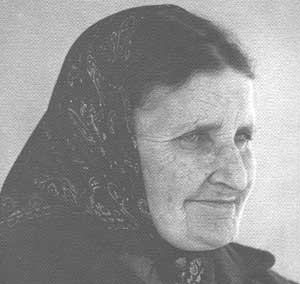
\includegraphics[scale=0.25]{gambar/simma.jpg}
\caption{\scriptsize\mbox{Maria Simma (1915-2004)}\normalsize}
\end{wrapfigure}

Saat ini, sangat sedikit yang diajarkan di kelas katekismus reguler tentang Api Penyucian, tentang penderitaan arwah-arwah agar benar-benar murni untuk dapat masuk ke dalam Kerajaan Surga. Namun Api Penyucian dan penderitaan arwah-arwah  adalah sangat nyata.

Sejak 1940 (ia saat itu berusia 25), seseorang yang istimewa, bernama Maria Simma, telah memiliki kunjungan rutin dari jiwa-jiwa di Api Penyucian untuk menjelaskan penderitaan mereka dan untuk meminta doa dan Misa agar dibebaskan dari Api Penyucian. Uskup setempat dan pastor paroki mengatakan bahwa ia boleh membuat kunjungan ini dikenal selama tidak ada kesalahan teologis.

Suatu hari, Suster Emmanuel Maillard, seorang biarawati Perancis yang menjalankan tugas kerasulan dan mendukung Penampakan Bunda Maria di Medjugorje, menemukan buku Maria Simma, yang berjudul \textit{The Souls in Purgatory told Me...} yang berupa mengenai arwah-arwah di Api Penyucian dan membacanya dengan penuh minat: ``Saya sungguh terpesona karena isinya menyangkut kesaksian-kesaksian baru-baru ini dan juga menjelaskan dengan baik tentang doktrin-doktrin Gereja Katolik tentang topik tersebut. Langsung, saya menulis kepada editor yang mengatakan kepada saya bahwa Maria Simma masih hidup. Dengan cepat, saya menghubungi dia, dan dia setuju untuk bertemu saya untuk menjawab pertanyaan saya, yang banyak!''

Wawancara ini berlangsung tahun 1997 di rumah Maria di Sonntag, sebuah desa yang sangat indah di Pegunungan Vorarlberg di Austria. Berikut ini adalah kutipan dari wawancara Suster Emmanuel (SE) dari Medjugorje dengan Maria Simma (MS), diambil dari sebuah buku kecil berjudul: \textit{The Amazing Secret of the Souls in Purgatory}, yang diterbitkan oleh Queenship Publishing Co, PO Box 220, Goleta, CA 93116, USA 

\noindent{\textit{(Catatan: Maria Simma meninggal pada 16 Maret 2004, di Sonntag, pada usia 89.)}}


\subsection*{PERTAMA KALINYA}
\newcommand{\BSE}[1]{\begin{itemize} \item[SE:] \textbf{#1} \end{itemize}}
\newcommand{\BMS}[1]{\begin{itemize} \item[MS:] \textit{#1} \end{itemize}}

\BSE{Maria, bisakah Anda menceritakan kepada kami bagaimana Anda pertama kali dikunjungi oleh arwah dari Api Penyucian?} 
\BMS{Ya, waktu itu tahun 1940. Suatu malam, sekitar jam 3 atau 4 pagi, saya mendengar seseorang masuk ke dalam kamar tidur saya. Hal itu membuat saya terbangun. Saya mencari-cari siapa gerangan yang dapat masuk ke dalam kamar tidur saya.}

\BSE{Apakah Anda ketakutan?}
\BMS{Tidak, saya tidak takut sama sekali. Bahkan sewaktu saya masih kecil, ibu saya mengatakan bahwa saya anak yang spesial karena saya tidak pernah merasa takut.}

\BSE{Jadi, malam itu... ceritakanlah kepada kami!}
\BMS{Saya melihat seorang yang sama sekali tidak saya kenal. Dia berjalan bolak-balik secara perlahan. Saya berseru keras kepadanya: "Bagaimana Anda dapat masuk kesini? Pergilah!" Tetapi dia terus berjalan dengan tidak sabar disekeliling kamar tidur, seolah-olah dia tidak mendengar perkataan saya. Jadi saya kembali bertanya: "Apa yang sedang Anda lakukan?" Tetapi karena dia tetap tidak memberi jawaban, saya turun dari ranjang dan mencoba menjamahnya, tetapi saya hanya menjamah udara kosong. Tidak ada apa-apa disana. Jadi saya kembali ke ranjang, tetapi kembali saya mendengarnya berjalan bolak-balik.
\\
Saya membayangkan bagaimana saya bisa melihat lelaki ini tetapi saya tidak dapat menjamahnya. Saya bangkit kembali untuk mencoba memegang orang itu dan menghentikan dia; kembali saya hanya merasakan kekosongan belaka.
\\
Bingung, saya lantas kembali ke ranjang. Dia tidak muncul kembali, tetapi saya tidak dapat kembali tidur. Hari berikutnya setelah Misa, saya menemui pembimbing spiritual saya dan menceritakan segalanya kepadanya. Dia berkata bahwa jika hal ini terulang kembali, saya jangan bertanya, "Siapakah Anda?" melainkan "Apa yang Anda inginkan dari saya?"
\\
Malam berikutnya orang tersebut muncul kembali, jelas-jelas orang yang sama. Saya bertanya kepadanya "Apa yang Anda inginkan dari saya?" Dia menjawab: "\textbf{Rayakan tiga Misa Kudus bagi saya dan saya akan dibebaskan}."
Jadi saya mengerti bahwa ia adalah arwah di Api Penyucian. Pembimbing spiritual saya menegaskan hal ini.
\\
Dia juga menasehatkan agar saya jangan mengusir jiwa-jiwa yang malang tersebut, tetapi menerima mereka dengan segala kemurahan hati apapun yang mereka minta dari saya.}

\BSE{Dan setelah itu, apakah kunjungan-kunjungan itu berlanjut?}

\BMS{Ya. Selama beberapa tahun, hanya ada tiga atau empat arwah, semua di bulan November. Setelah itu, ada lebih banyak lagi.}

\subsection*{SEBUAH LUKA-KASIH}

\BSE{Apa yang diminta oleh arwah-arwah ini dari Anda?}
\BMS{Pada umumnya mereka minta dirayakan Misa-misa Kudus dan seseorang hadir pada Misa-misa tersebut; mereka meminta supaya doa-doa Rosario diucapkan dan juga agar seseorang melakukan Perhentian-perhentian Jalan Salib.}

Pada saat ini, suatu pertanyaan utama muncul: Sesungguhnya apakah Api Penyucian tersebut? Saya akan katakan bahwa itu adalah merupakan ciptaan Tuhan yang luar biasa. Ijinkan saya untuk memberikan Anda suatu gambaran dari saya sendiri. Misalkan suatu ketika sebuah pintu terbuka dan sesosok mahluk muncul, sangat luar biasa indah, keindahan yang tidak pernah ada di dunia. Anda terpesona, terpesona oleh mahluk cahaya yang indah ini, terlebih-lebih mahluk tersebut menunjukkan bahwa ia sangat mengasihi Anda. Anda tidak pernah membayangkan kalau Anda begitu dikasihi. Anda juga merasakan bahwa Anda punya keinginan besar untuk menjadi satu dengannya. Dan api cintakasih yang menyala dalam hati Anda mendorong Anda untuk menyerahkan diri Anda kedalam tangannya.

Tetapi tunggu dulu -- Anda sadar pada saat ini bahwa Anda belum mandi selama berbulan-bulan dan Anda bau sekali; hidung Anda penuh lendir, rambut Anda kotor dan lengket, ada noda besar di baju Anda dan lain sebagainya. Jadi Anda berkata kepada diri sendiri, ``Saya tidak bisa memberikan diri saya dengan kondisi seperti ini. Pertama saya harus pergi dan membersihkan diri: mandi bersih, lantas saya akan segera kembali.''

Tetapi cintakasih yang telah lahir dalam hati Anda begitu kuatnya, menyala-nyala, begitu dahsyat, sehingga penundaan ini demi untuk membersihkan diri ini menjadi sangat tidak tertahankan. Dan rasa sakit karena absennya Anda, meski jika hanya untuk selama beberapa menit saja, adalah luka yang hebat di dalam hati, proporsional terhadap intensitas pernyataan cintakasih -- ini adalah sebuah ``luka cinta-kasih''.

Api Penyucian tepat seperti ini. Sebuah penundaan yang diakibatkan oleh ketidak-sucian kita sendiri, sebuah penundaan sebelum menerima Tuhan, sebuah luka cintakasih yang menyebabkan penderitaan yang luar biasa, sebuah penungguan, sebuah nostalgia cintakasih. Pembakaran inilah tepatnya, kerinduan ini yang membersihkan kita dari apapun yang masih kotor dalam diri kita. Api Penyucian adalah suatu tempat keinginan, keinginan yang dahsyat akan Tuhan, kerinduan akan Tuhan yang telah kita kenal, karena kita telah menyaksikannya, tetapi dengan siapa kita belum dipersatukan.

Sekarang saya akan menanyakan kepada Maria untuk menjelaskan sebuah poin yang mendasar:

\BSE{Maria, apakah jiwa-jiwa di Api Penyucian memiliki, setidak-tidaknya, suka cita dan pengharapan di tengah-tengah penderitaan mereka}

\BMS{Ya. Tidak ada arwah yang ingin kembali dari Api Penyucian ke dunia. Mereka memiliki pengetahuan yang jauh melebihi yang kita miliki. Mereka sungguh tidak dapat memutuskan untuk kembali ke kegelapan dunia.}

Disini kita melihat perbedaan dari penderitaan yang kita kenal di dunia. Di Api Penyucian, meskipun penderitaan yang dialami oleh jiwa begitu hebatnya, ada kepastian akan hidup selamanya dengan Tuhan. Ini adalah kepastian yang tidak tergoyahkan. Kesukacitaannya lebih besar daripada penderitaan. Tidak ada apapun di bumi yang dapat membuat mereka ingin kembali kesana, dimana seseorang tidak pernah dapat yakin akan segala sesuatu.

\BSE{Maria, dapatkan Anda menceritakan kepada kami sekarang jikalau Tuhanlah yang mengirimkan arwah seseorang kedalam Api Penyucian, atau apakah arwah tersebut sendiri yang memutuskan untuk pergi ke sana?}

\BMS{Arwah itu sendiri yang ingin pergi ke Api Penyucian, demi untuk menjadi murni sebelum dapat masuk ke Surga.}

Arwah-arwah di Api Penyucian menurut pada kehendak Allah sepenuhnya, mereka bersukacita atas kebaikan, mereka menginginkan yang terbaik bagi kita dan mereka sangat mengasihi: mereka mengasihi Allah dan mereka juga mengasihi kita. Mereka dipersatukan dengan sempurna dengan Roh Allah, terang Allah.


\BSE{Maria, pada saat ajal, apakah seseorang melihat Allah secara sepenuhnya ataukah dengan cara tidak tampak jelas?}

\BMS{Dengan cara tidak tampak jelas, tetapi, pada saat yang sama, dengan terang yang sedemikian rupa sehingga ini cukup untuk menimbulkan kerinduan yang dahsyat.}

Sesungguhnya, terang yang begitu gemilang dibandingkan dengan kegelapan dunia. Dan masih bukan apa-apa dibandingkan dengan terang seutuhnya yang jiwa akan ketahui ketika jiwa tersebut tiba di Surga. Di sini kita bisa merujuk pada "pengalaman-pengalaman orang yang nyaris mati." Jiwa seseorang begitu tertariknya kepada terang ini sehingga sungguh merupakan suatu penderitaan baginya untuk kembali ke bumi ke dalam tubuhnya setelah pengalaman ini.

\subsection*{KEMURAHAN HATI MENEBUS SEJUMLAH DOSA-DOSA}

\BSE{Maria, dapatkan Anda menceritakan kepada kami apa peran Bunda Maria terhadap jiwa-jiwa di Api Penyucian?}

\BMS{Dia sering datang untuk menghibur mereka dan untuk memberitahu mereka bahwa mereka telah banyak melakukan hal-hal baik. Dia memberi mereka semangat.}

\BSE{Apakah ada hari-hari tertentu dimana Bunda Maria membebaskan mereka?}

\BMS{Diantara semuanya, Hari Natal, Hari Semua Orang Kudus, Hari Jumat Agung, Hari Raya Maria Diangkat ke Surga, dan Hari Raya Yesus Naik ke Surga.}

\BSE{Maria, mengapa seseorang masuk kedalam Api Penyucian? Dosa-dosa manakah yang paling membawa ke dalam Api Penyucian?}

\BMS{Dosa-dosa terhadap kemurahan hati, terhadap kasih kepada sesama, kebekuan hati, permusuhan, fitnah, pengrusakan nama baik seseorang - segala hal-hal semacam ini.}

\BSE{Mengatakan hal-hal yang buruk dan fitnah adalah diantara noda-noda yang terburuk yang membutuhkan pemurnian yang lama?}

\BMS{Ya.}

Disini, Maria memberi sebuah contoh yang sungguh mengejutkan dia yang ingin saya ceritakan kepada Anda.

Dia telah diminta untuk mencari tahu jikalah seorang wanita dan seorang pria berada di Api Penyucian.

Betapa terkejutnya mereka yang menanyakan hal tersebut, karena wanita tersebut telah berada di Surga sedangkan yang pria masih berada di Api Penyucian. Sesungguhnya, wanita ini meninggal ketika sedang menjalani aborsi, sementara sang pria seringkali pergi ke gereja dan tampaknya menjalani hidup dengan baik dan taat.

Jadi Maria mencari informasi lebih jauh, dan berpikir bahwa dia telah salah duga - tetapi, tidak, ternyata memang benar demikian adanya. Mereka berdua meninggal pada saat yang bersamaan, tetapi sang wanita sempat bertobat secara mendalam, dan sangat rendah hati, sementara sang pria seringkali mengkritik semua orang; dia selalu memprotes dan mengatakan hal-hal buruk tentang orang lain. Inilah sebabnya mengapa dia berada lama di Api Penyucian. Dan Maria menyimpulkan: "\textit{Kita tidak bisa menilai dari penampilan}."

Dosa-dosa lain terhadap kemurahan-hati adalah penolakan kita terhadap orang-orang tertentu yang tidak kita sukai, penolakan kita untuk berdamai, penolakan kita untuk memaafkan, dan segala kegetiran yang kita simpan dalam hati.

Maria juga menggambarkan poin ini dengan sebuah contoh yang lain untuk kita pikirkan. Ini kisah tentang seorang wanita yang sangat ia kenal. Wanita ini meninggal dan berada di Api Penyucian, di Api Penyucian yang paling mengerikan, dengan kesengsaraan yang paling hebat. Dan ketika dia datang untuk menemui Maria, dia menjelaskan mengapa sebabnya: dia mempunyai seorang teman wanita; diantara mereka muncul suatu permusuhan yang hebat, yang disebabkan oleh dirinya sendiri. Dia telah memelihara permusuhan ini tahun demi tahun, meskipun sahabatnya telah berulang-kali meminta untuk berdamai, untuk kembali bersahabat. Tetapi setiap kali dia menolak. Ketika dia jatuh sakit parah, dia terus menutup hatinya, menolak berdamai yang ditawarkan oleh kawannya, sampai kematiannya. Saya percaya contoh ini adalah contoh yang penting mengenai kebencian yang dipelihara. Dan kata-kata kita sendiri juga, bisa merusak: kita tidak akan pernah bisa menekankan betapa suatu kata yang kritis atau pahit bisa sungguh-sungguh membunuh - tetapi juga, sebaliknya, betapa sebuah kata bisa menyembuhkan.

\BSE{Maria, harap ceritakan kepada kami: siapakah orang-orang yang punya kesempatan terbesar untuk langsung masuk ke Surga?}

\BMS{Mereka yang mempunyai hati yang baik terhadap semua orang. Cintakasih menebus sejumlah besar dosa-dosa.}

Ya, Santo Paulus sendiri mengatakan hal ini!

\BSE{Apakah cara-cara yang bisa kita lakukan di dunia untuk menghindari Api Penyucian dan langsung masuk ke Surga?}

\BMS{Kita harus melakukan banyak hal bagi jiwa-jiwa di Api Penyucian, oleh karena mereka menolong kita pada gilirannya. Kita harus memiliki banyak kerendahan hati; ini adalah senjata terbesar melawan kejahatan, melawan Yang Jahat. Kerendahan hati mengusir kejahatan.}

Saya tidak bisa menghindar untuk menceritakan sebuah kesaksian yang sangat indah oleh Father Berlioux (yang menulis sebuah buku yang bagus tentang jiwa-jiwa di Api Penyucian), mengenai bantuan yang diberikan oleh jiwa-jiwa ini terhadap orang-orang yang membebaskan mereka melalui doa-doa dan pengorbanan mereka.

Dia mengisahkan tentang seorang yang membaktikan dirinya demi jiwa-jiwa yang malang, dimana dia telah mengkonsekrasikan hidupnya demi membantu membebaskan mereka.

\textit{
\begin{quote}
``Pada saat menjelang ajalnya, wanita ini diserang dengan ganas oleh iblis yang melihat dia lepas dari cengkeramannya. Tampaknya seluruh jurang bersatu melawan dia, mengelilinginya dengan pasukan neraka. 
Wanita yang menjelang ajal ini memberontak dengan susah payah untuk beberapa waktu ketika tiba-tiba dia melihat masuk kedalam apartemennya sejumlah arwah-arwah tak dikenal yang bercahaya menyilaukan indah, yang membuat iblis melarikan diri dan, mendekati ranjang wanita tersebut, berbicara kepadanya dengan dukungan semangat surgawi dan penghiburan. Dengan tarikan nafasnya terakhir wanita itu bertanya, dengan penuh sukacita, dia menangis: 'Siapakah kalian? Siapakah kalian, oh, kalian yang sangat baik terhadap saya?'
"Para pengunjung yang baik hati tersebut menjawab: 'Kami adalah penghuni Surga, yang atas pertolonganmu telah dipimpin kedalam Kebahagian Surgawi. Dan kami pada gilirannya datang dengan penuh rasa terima kasih untuk menolong Anda menyeberangi batas kekekalan dan menyelamatkan Anda dari tempat yang sengsara ini untuk membawamu kedalam sukacita Kota yang Kudus.'
"Atas kata-kata tersebut, sebuah senyuman muncul pada wajah wanita yang sekarat tersebut, matanya menutup dan diapun tertidur dalam damai Tuhan Yesus. Jiwanya, murni seperti merpati, dipersembahkan kepada Raja segala raja, mendapat banyak pelindung dan pembela sebanyak jiwa-jiwa yang telah ia tolong dulunya, dan ia layak atas kemuliaan, ia masuk dengan kemenangan, ditengah-tengah sorak dan berkat dari mereka yang telah ia tolong bebaskan dari Api Penyucian. Semoga kita, suatu hari, mendapat kebahagiaan yang serupa.''
\end{quote}
}

Jiwa-jiwa yang dibebaskan atas pertolongan doa-doa kita sangat berterima kasih: mereka menolong kita dalam hidup kita; bisa kita rasakan. Saya dengan tegas merekomendasikan supaya Anda mengalaminya sendiri! Mereka sungguh-sungguh menolong kita; mereka tahu kebutuhan-kebutuhan kita dan memintakan banyak rahmat bagi kita.

\BSE{Maria, saya memikirkan tentang Pencuri yang Bertobat yang berada di sebelah Yesus di Salib. Saya sungguh ingin mengetahui apakah yang dilakukannya sehingga Yesus menjanjikannya bahwa hari itu juga seterusnya dia akan berada di dalam Kerajaan bersama Dia?}

\BMS{Pencuri itu dengan rendah hati menerima penderitaannya, mengatakan bahwa hal itu adil. Dan dia menyemangati pencuri yang satunya lagi untuk menerima penderitaannya juga. Dia takut akan Allah, yang berarti memiliki kerendahan hati.}

Suatu contoh lain yang bagus dikisahkan oleh Maria Simma menunjukkan betapa sebuah tindakan yang baik menebus sebuah hidup yang penuh dosa. Mari dengarkan dari Maria sendiri:

\begin{quote}
\textit{Saya kenal seorang lelaki muda yang kira-kira berumur 20 tahun, di desa yang berdekatan. Desa tempat tinggal orang ini telah ditimpa bencana serentetan tanah longsor yang telah membunuh sejumlah besar penduduk. Suatu malam, orang muda ini berada di rumah orang-tuanya ketika dia mendengar tanah longsor tepat di sebelah rumahnya. Dia mendengar jeritan-jeritan yang memekakkan, menyayat hati, 'Selamatkan kami! Datanglah, selamatkanlah kami! Kami terjebak di bawah longsoran ini!'
\\
Melompat, bangkitlah dia dari ranjangnya dan tergesa-gesa turun ke bawah untuk menyelamatkan orang-orang ini. Ibunya telah mendengar jeritan-jeritan tersebut dan mencegahnya untuk pergi; dia menghalang di depan pintu dan berkata 'Tidak! Biarkan orang-orang lain yang menolong mereka, jangan selalu kita! Terlalu berbahaya di luar, saya tidak ingin ada lagi yang meninggal!' 
Tetapi dia, karena telah terdorong oleh jeritan-jeritan ini, sungguh ingin menolong orang-orang tersebut; dia mendorong ibunya kesamping. Dia berkata: 'Ya! Saya pergi, saya tidak dapat membiarkan mereka mati seperti ini!' Dia keluar, dan lantas dia sendiri di tengah jalan, tertimbun tanah longsor dan mati terbunuh.
\\
Tiga hari setelah kematiannya, dia datang untuk mengunjungi saya, pada malam hari, dan dia berkata kepada saya: 'Rayakanlah tiga Misa Kudus untuk saya; olehnya, saya akan dibebaskan dari Api Penyucian.' Saya pergi untuk memberitahu sanak keluarga dan teman-temannya; mereka tercengang ketika mengetahui bahwa hanya setelah tiga kali Misa Kudus, dia akan dibebaskan dari Api Penyucian. Sahabat-sahabatnya berkata: 'Oh, saya tidak akan ingin untuk menjadi dirinya pada saat kematian, jika Anda tahu hal-hal buruk yang telah dia lakukan selama ini!'
\\
Tetapi orang muda ini berkata kepada saya: 'Anda tahu, saya telah melakukan tindakan kasih yang tulus dengan membahayakan diri saya sendiri demi orang-orang tersebut; atas hal inilah Tuhan menerima saya begitu cepat kedalam SurgaNya. Ya, belaskasihan menebus sejumlah besar dosa-dosa...'}
\end{quote}

Kisah ini menunjukkan kepada kita bahwa belaskasihan, satu tindakan kasih yang diberikan secara cuma-cuma, telah cukup untuk memurnikan jiwa orang muda ini dari kehidupan yang immoral; dan Tuhan Yesus telah mempergunakan sebaik-baiknya dari satu saat cintakasih tersebut. Maria bahkan menambahkan bahwa orang muda ini tidak akan pernah lagi mendapat kesempatan untuk mempersembahkan tindakan kasih yang sedemikian besar, dan bisa bertambah buruk. Tuhan dalam belaskasihNya, mengambil nyawa orang tersebut ketika ia muncul di hadapan Allah pada kondisinya yang terbaik, terbersih, oleh karena tindakan kasih tersebut.

Sangat penting kiranya, pada saat menjelang ajal, untuk menyerahkan diri kepada kehendak Allah.

Maria mengatakan kepada saya tentang kasus seorang ibu atas empat anak yang menjelang ajal. Bukannya memberontak dan khawatir, dia berkata kepada Tuhan: ``Saya menerima ajal, sepanjang itu adalah kehendakMu, dan saya akan menaruh nyawa saya ke dalam tanganMu. Saya mempercayakan anak-anak saya kepadaMu dan saya tahu bahwa Engkau akan menjaga mereka.''

Maria berkata bahwa, karena kepercayaannya yang besar terhadap Tuhan, wanita ini langsung masuk ke Surga dan terhindar dari Api Penyucian.

Oleh karena itu, kita sungguh dapat mengatakan bahwa kasih, kerendahan hati, dan menurut pada kehendak Allah adalah tiga kunci emas untuk dapat langsung masuk ke Surga.


\sumber{The Secret of the Poor Souls in Purgatory\\
An interview with Maria Simma of Austria\\
http://www.michaeljournal.org/simma.htm}

\sumber{Rahasia Arwah-arwah di Api Penyucian\\
Wawancara Suster Emmanuel dari Medjugorje dengan visionari Maria Simma\\
http://www.gerejakatolik.net/artikel/rahasia.htm}
\setlength{\parindent}{1cm}

\normalsize
\chap{Datanglah Kerajaan-Mu}
\small
``Mbak Wid, bagaimana keadaan bapak?'', tanya Johanes Sukendro teman kuliah suamiku Agung Laksono disaat aku sedang bertugas sebagai perawat di bagian ICU di sebuah rumah sakit swasta di Jogjakarta. 

``Belum ada peningkatan mas, penyakit bapak menurut dokter sudah berat.'', jawabku turut merasa prihatin. ``Doakan Mas Jo, semoga Tuhan berkenan memberi  kesembuhan kepada bapak. Dokter dan kami perawat akan berusaha semampu kami.'', ujarku selanjutnya. 

``Terima kasih mbak Wid, kami tetap berdoa memohon kesembuhan untuk bapak.'', ujar Jo sambil menyalamiku kemudian Jo pergi menunggu diluar.

Aku pergi menghampiri ranjang Pak Widi (nama bapaknya Jo), aku melihat ada kegelisahan pada diri Pak Widi. Beliau tidak bisa memejamkan mata seperti hari-hari lalu. Melihat kegelisahan yang beliau alami, aku mencoba mendekat dan menanyakannya. Ketika aku datang dan menyentuhnya, Pak Widi memandangku dalam-dalam. 

``Suster \ldots mengapa suster menjadi perawat?'', tanya Pak Widi tiba-tiba. Aku sendiri terkejut dengan pertanyaan itu. Semula aku akan menanyakan tentang kegelisahannya, tiba-tiba disodori pertanyaan diluar dugaanku. Aku tidak yakin dengan pertanyaan itu. Jangan-jangan Pak Widi ini bicara diluar kendali.

``Bagaimana Pak?',' tanyaku ulang.

``Suster \ldots Mengapa Suster menjadi perawat?'', Pak Widi mengulangi pertanyaannya. Yakin akan kesungguhan pertanyaan itu, maka aku mencoba mengisahkan pengalamanku, selain itu aku ingin menghiburnya, mungkin dengan mendengarkan ceritaku kegelisahannya bisa berkurang dan beliau bisa tidur tenang, ternyata tidak demikian.

``Pak \ldots mengapa bapak belum juga tidur. Bapak memikirkan apa?'', tanyaku lembut.
Pak Widi hanya diam saja. Matanya masih terbuka lebar dan menatap padaku. Aku menjadi bingung. Apa yang harus aku lakukan?

``Pak \ldots ini sudah jam dua pagi, bapak istirahat ya!'', ajakku.

Pak Widi tetap diam. Sementara bunyi monitor pasien lain berbunyi. Aku tidak beranjak, kulihat teman perawat lain menanganinya. Monitor dan erangan pasien memang menjadi perhatian khusus bagi kami semua yang bertugas pada waktu itu.
Kembali perhatianku kuarahkan pada Pak Widi.

``Pak, lebih baik bapak berdoa, supaya bapak bisa tenang dan bapak bisa tidur dengan tenang. Saya akan berdoa untuk bapak menurut cara yang saya imani. Bapak juga demikian.'' ujarku memohon.

Tiba-tiba tangan Pak Widi yang kekar itu meraih tanganku, katanya, ``Suster \ldots Berdoalah disamping saya.''

``Baik, Pak. Saya akan berdoa untuk bapak. Bapak sendiri berdoa menurut cara yang bapak anut.'' 

Aku memilih berdoa Bapa Kami. Baru beberapa kata kumulai, Pak Widi berkata, ``Suster \dots keras sedikit. Saya ingin dengar.''
Kuawali lagi doa Bapa Kami. ``Bapa kami yang ada di surga, dimuliakanlah nama-Mu. Datanglah kerajaan-Mu.''

Tiba-tiba Pak Widi menirukan yang kuucapkan, ``datanglah kerajaan-Mu''

``Tit \ldots tit \ldots Tit \ldots '' suara monitor pernapasan dan jantung itu mendadak berhenti besamaan dengan suara Pak Widi menirukan ucapanku, ``datanglah kerajaan-Mu.''

Aku cepat-cepat bangkit dan memanggil teman-teman. Aku dan teman-teman pun kemudian sibuk untuk menangani Pak Widi. Sementara ada teman yang lain memanggil dokter jaga untuk membantu menyelamatkannya. Setelah sepuluh menit kami berjuang untuk menyelamatkan Pak Widi, ternyata kami tidak berhasil. Tepat pukul 02.30 WIB Pak Widi dinyatakan meninggal dunia.

Meski kulihat wajahnya begitu tenang, namun aku merasa kehilangan. Pak Widi walaupun baru tiga hari aku mengenalnya, aku merawatnya dengan penuh kasih, apalagi beliau adalah bapak dari Jo sahabat suamiku, aku merasa seperti merawat orangtuaku sendiri. Tanpa kusadari airmataku meleleh jatuh kepipiku. Aku merasa bingung dan merasa bersalah kepada Mas Jo, karena sama sekali belum peka dengan tanda-tanda akan kematian.

Aku segera menghubungi suamiku dan menghubungi Mas Jo, mengabarkan kepergian Pak Widi ke kerajaan Allah dengan perasaan merasa bersalah. Suamiku dan Mas Jo segera datang ke rumah sakit.

``Maafkan saya, Mas Jo \ldots saya sungguh merasa bersalah.'', ujarku dengan diiringi lelehan air mata.

``Sudah kehendak Allah yang Mahakuasa, Mbak Wid. Terima kasih mbak Wid  mau merawat dan mendampingi  bapak. Tidak perlu merasa bersalah.'', kata Jo tegar. 

Kemudian aku menceritakan proses kejadiannya hingga Pak Widi pergi ke kerajaan Allah kepada Mas Jo dan suamiku.

``Syukur kepada Allah. Sungguh rahmat yang luar biasa bagi bapak. Hatiku tenang akan kepergian bapak.'', ujar Jo dengan rasa penuh syukur. 

\begin{flushright}
\textit{Medio Oktober’2011 \\Bravo Sierra}
\end{flushright}
\normalsize
\chap{Kerahiman Ilahi}

 ``Gung, kamu kan tahu kalo bapakku masih seorang muslim walaupun ibuku sudah katolik. Coba kamu lihat isi dompet milik bapakku'', kata Jo sambil menyodorkan sebuah dompet lusuh kepadaku. Dengan rasa heran aku menerima dompet itu dan membukanya.    
 
``Isinya ada uang dua ratus ribu rupiah, KTP, SIM C dan foto bu Widi.'', ujarku heran.

``Coba kamu rogoh selipan dibelakang KTP, Gung.'', kata Jo. Aku merogoh selipan dibelakang KTP ternyata ada gambar Tuhan Yesus dan gambar Bunda Maria dan sebuah kertas lipatan. Aku membuka kertas lipatan itu dan membacanya:
\begin{quote}
\textit{
KepadaMu ya Tuhan, kuangkat jiwaku; Allahku, kepadaMu  aku percaya; janganlah kiranya aku mendapat malu; janganlah musuh-musuhku bersuka ria atas aku. Ya, semua orang yang menantikan Engkau takkan mendapat malu; yang mendapatkan malu adalah mereka yang berbuat khianat dengan tidak ada alasannya. Bawalah aku berjalan dalam kebenaranMu dan ajarlah aku, sebab Engkaulah Allah yang menyelamatkan aku, Engkau kunanti-nantikan sepanjang hari. Ingatlah segala rahmatMu dan kasih setiaMu, ya Tuhan, sebab itu sudah ada sejak purbakala. Dosa-dosaku pada waktu muda dan pelanggaran-pelanggaranku janganlah Kau ingat, tetapi ingatlah kepadaku sesuai dengan kasih setiaMu, oleh karena kebaikanMu, ya Tuhan. Tuhan itu baik dan benar; sebab itu Ia menunjukkan jalan kepada orang yang sesat. Ia membimbing orang-orang yang rendah hati menurut hukum, dan Ia mengajarkan jalanNya kepada orang-orang yang rendah hati. Segala jalan Tuhan adalah kasih setia dan kebenaran bagi orang yang berpegang pada perjanjianNya dan peringatan-peringatanNya. Oleh karena namaMu, ya Tuhan, ampunilah kesalahanku, sebab besar kesalahan itu. Siapakah orang yang takut akan Tuhan? Kepadanya Tuhan menunjukkan jalan yang harus dipilihnya.}
\end{quote}



``Syukur kepada Allah. Ini adalah ayat-ayat Mazmur.'', ujarku sambil menatap wajah Jo yang penuh senyum gembira.

``Tapi Gung, walaupun ibuku sudah mengetahui hal ini, ibuku tetap memintaku untuk mengadakan upacara doa pelepasan dan pemakaman jenazah bapak dengan ritual secara agama Islam. Menurutmu bagaimana?'', tanya Jo. 


``Seharusnya begitu Jo, karena masyarakat di kampung ini mengetahui Pak Widi adalah seorang muslim. Janganlah kamu khawatir, Tuhan pasti mencari domba-dombaNya yang hilang.'', kataku sambil menepuk bahu sahabatku.

Para pelayat mulai berdatangan,  upacara doa pelepasan jenazah Pak Widi dilakukan secara agama Islam, hingga sampai di pemakaman.  Karena profesiku seorang kuli tinta tanpa sadar aku sering mengambil foto dengan camera HP ku. Ketika  jenazah Pak Widi dimasukkan ke liang makam, aku mencoba mengambil gambar (foto) nya, tapi entah mengapa kok tiba-tiba pencetan/tombol pengambil foto macet, tidak bisa di pencet seperti macet. Berulang kali aku mencoba memencet-mencet tombol pengambil  foto sampai akhirnya aku berhasil memencet mengambil foto jenazah Pak Widi di liang makam. Sampai acara pemakaman selesai cukup banyak foto yang berhasil aku ambil.

Sesampai di rumah, karena kebiasaanku sebagai kuli tinta, aku melihat kembali hasil foto-foto  yang berhasil  aku ambil. Hanya ada satu yang aneh yaitu foto jenazah Pak Widi di liang makam tidak mau keluar gambarnya. 

Esok harinya aku mencetak foto-foto pemakaman Pak Widi melalui komputerku. ``Ya Tuhan!!!'', seruku seorang diri. Foto jenazah Pak Widi di liang makam tercetak. Tampak samar-samar seperti  ada 2 orang malaikat kecil disamping kepala Pak Widi dengan penuh suka cita.  Kuambil semua hasil cetak  foto-foto itu lalu kumasukkan ke dalam tas punggungku. Bergegas kupacu sepeda motorku menuju kerumah Jo.

`` Jo, coba kamu lihat foto ini.'', ujarku sambil menyodorkan foto jenazah Pak Widi di liang makam. 

``Ada apa Gung?  Ini kan foto jenazah bapak di liang makam.'', kata Jo keheranan. ``Coba kamu lihat baik-baik foto itu. Di samping kepala bapak tampak samar-samar ada 2 malaikat kecil'', kataku sambil menunjukkan letaknya. Lalu aku ceritakan kejadian pengambilan foto itu terasa sangat aneh karena aku merasa HP ku tidak rusak.

Waktu terus berputar, 40 hari berlalu setelah Pak Widi berpulang kehadirat Tuhan. Jo mengajakku mengunjungi makam Pak Widi bapaknya. Sesampai di pemakaman  ada seorang pemuda sedang berdoa di sebuah makam tepat di samping makam Pak Widi. Kami berdua berjalan menuju makam Pak Widi dan menyapa pemuda itu.

``Selamat pagi Mas.'' Sapaku ramah. 

``Selamat pagi pak.'' kata pemuda itu. Kami lalu saling berkenalan dan saling bercerita tentang orang-orang yang dikasihi telah menghadap sang khalik.

``Bapak seorang katolik? Boleh saya turut mendoakan arwah beliau?'' tanya pemuda itu ternyata melihat kalung salib bercorpus yang dipakai Jo.

``Benar Romo. Terima kasih Romo berkenan mendoakan arwah Pak Widi.'', ujarku cepat tanggap karena aku melihat tanda salib pada krah baju yang dipakai pemuda itu. 

\begin{quote}
\textit{
Allah Bapa pemilik bumi dan Surga,\\
Engkau telah memanggil salah seorang putra-Mu, Bapak Widiatmoko,
 agar duduk di sisi-Mu, bersama para kudus. \\
Bersanding dengan Putra-Mu terkasih,\\ Tuhan Yesus Kristus.\\
 Ampunilah segala dosa dan kesalahannya, bebaskan dia dari hukuman dan denda surgawi, sebab dia sudah mengimani Putra-Mu sebagai Juru selamat sejati.\\
 Bunda Maria, Bunda Segala Bangsa, hantarkan putramu ini untuk menghadap Putramu, Tuhan Yesus Kristus, yang bersama Allah Bapa dan Roh Kudus, hidup dan bertahta, kini  dan sepanjang segala abad. \\Amin.}
\end{quote}

\begin{flushright}
\textit{Medio Oktober 2011 \\Bravo Sierra}
\end{flushright}
\normalsize
\vfill
\noindent{\framebox{\parbox{10cm}{\centering\emph{
``Kehidupan yang benar dan sejati ialah:\\
Bapa, melalui Putra, dan dalam Roh Kudus,
mencurahkan anugerah-anugerah surgawi-Nya
kepada segala sesuatu tanpa kecuali.\\
Melalui kerahiman-Nya, kita manusia juga menerima
janji hidup ilahi yang tak dapat diragukan lagi''\\ 
(Santo Cyrillus dari Yerusalem)}}}}


\chap{Sesuatu Tidak Selalu Kelihatan Sebagaimana Adanya}

\small
Dua orang malaikat berkunjung ke rumah sebuah keluarga kaya. Keluarga itu sangat kasar dan tidak mengijinkan kedua malaikat itu bermalam di ruang tamu yang ada di rumahnya, malaikat tersebut ditempatkan pada sebuah kamar berukuran kecil yang ada di basement. Ketika malaikat itu hendak tidur, malaikat yang lebih tua melihat bahwa dinding basement itu retak. Kemudian malaikat itu memperbaikinya sehingga retak pada dinding basement itu lenyap dan ketika malaikat yang lebih muda bertanya mengapa ia melakukan hal itu, malaikat yang lebih tua menjawab, “sesuatu tidak selalu kelihatan sebagaimana adanya''.

Malam berikutnya, kedua malaikat itu beristirahat di rumah seorang petani dan istrinya yang miskin tetapi sangat ramah. Setelah membagi sedikit makanan yang ia punyai, petani itu mempersilahkan kedua malaikat untuk tidur di atas tempat tidurnya.

\begin{wrapfigure}{r}{1.5cm}
\centering

\includegraphics[scale=0.07]{gambar/malaikat.png}
\end{wrapfigure}

Ketika matahari terbit keesokan harinnya, malaikat menemukan bahwa petani itu dan istrinya sedang menangis sedih karena sapi mereka yang merupakan sumber pendapatan satu-satunya bagi mereka, terbaring mati. Malaikat yang muda merasa geram. Ia bertanya kepada malaikat yang lebih tua.
``mengapa kau membiarkan hal ini terjadi? Keluarga yang pertama memiliki segalanya, tapi engkau menolong menambalkan dindingnya yang retak. Keluarga ini hanya memliki sedikit, tetapi walaupun demikian mereka bersedia membaginya dengan kita. Mengapa engkau membiarkan sapinya mati?''

Malaikat yang lebih tua menjawab, ``sesuatu tidak selalu kelihatan sebaaimana adanya''.
``ketika kita bermalam di basement, aku melihat ada emas tersimpan di lubang dalam dinding itu. Karena pemilik rumah sangat tamak dan tidak bersedia membagi hartanya, aku menutup dinding itu agar ia tidak menemukan emas itu''.

 ``Tadi malam ketika kita tidur di ranjang petani ini, malaikat maut datang untuk mengambil nyawa istrinya, aku memberikan sapinya agar malaikat maut tidak jadi mengambil istrinya.''

\begin{wrapfigure}{l}{1cm}
\centering

\includegraphics[scale=0.09]{gambar/malaikat2.png}
\end{wrapfigure}

MEMANG, ``Terkadang Sesuatu Tidaklah Tampak Sebagaimana Kelihatannya''. Kadang-kadang itulah yang kita rasakan ketika berpikir bahwa sesuatu tidaklah seharusnya terjadi.

Jika kita punya iman, kita hanya perlu percaya bahwasanya semua hal yang terjadi adalah demi kebaikan kita. Kita tidak menyadari hal itu sampai saatnya tiba.

\sumber{``Sesuatu Tidak Selalu Kelihatan Sebagaimana Adanya.''\\
 www.renungan-harian-kita.blogspot.com.}
\normalsize
\chap{Aku Mencari Tuhan Tanpa Kartu Pos} 

\begin{wrapfigure}[11]{l}{2.75cm}
\centering
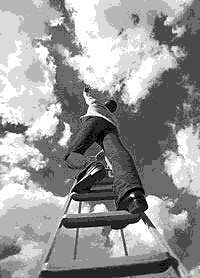
\includegraphics[scale=0.4]{gambar/aku-mencari-bw.jpg}
\end{wrapfigure}


Sebuah pesan di pintu mesin pendingin makanan. 
Tuhan pagi ini sengaja tak membangunkanku, ia hanya menempelkan secarik kertas:

"\textbf{ketika kau membaca ini, engkau telah terbangun}"


Lalu aku menuju meja makan, perut begitu lapar. Ketika aku membuka tudung saji, aku berharap Tuhan telah memasakkanku sepiring nasi goreng. Aku dapatkan secarik kertas di atas piring. Tertulis, "\textbf{ketika kau membaca ini, kau sudah kenyang}"

Di pintu lemari, akupun melihat sebuah kertas kecil, "\textbf{ketika kau membaca ini, hatimulah pakaianmu yang terindah}" Aku tahu, baju-bajuku telah membusuk di pojok kamar mandi.

Ketika aku membaca berbagai tulisan di dinding, laci, langit-langit dan pintu, tertulis, "\textbf{ketuklah, maka akan dibukakan}"

Ketika aku menyapa jalan, orang-orang yang berlalulalang, lampu merah dan asap-asap knalpot. Mereka lupa pada kata ``diam''. Melangkah seakan sudah menyatakan bahasa, bahwa mereka sedang diburu-buru hidup.

Aku mencari Tuhan tanpa kartu pos. Berharap Ia menuliskan pesan di badan bis-bis kota, di spanduk yang terbentang atau di kerumunan suara yang meneriakkan perutnya.

Aku mencari Tuhan dengan berkata-kata, dengan bertanya-tanya.
Aku mencari wajahnya dengan menatap mata-mata, senyum.
Aku menemukan jejaknya di sebuah sudut kota.

Kata mereka, “Tuhan pernah mampir dan selanjutnya pergi.”
"Mengapa tak kalian paksa saja ia tinggal di sini?"
"Kami rasa, masih banyak orang yang akan dijumpainya. Kami sudah kuat oleh kata-kata yang ditinggalkannya."

Aku terhenyak diam. Tuhan juga meninggalkanku pagi-pagi tadi.
Atau mungkin ia marah, ketika aku memperlakukannya tak pantas, memintanya untuk berjaga dikala tidur malamku bak seorang satpam, memintanya menghantarkanku selamat ke tujuan bagai seorang supir berpengalaman, meminta makanan, meminta rejeki, meminta jodoh, meminta naik pangkat, meminta \ldots meminta \ldots

"Di sini kami tak meminta. Karena kami tak mampu meminta padanya."

"Mengapa? Apakah kalian tak sadar, Ia mampu memberi apa yang kalian pinta."

"Kami tahu, Ia lebih tahu apa yang kami butuhkan. Tanpa diminta, Ia sudah melakukan.”

Ketika aku pulang tanpa bergandengan tangan dengan Tuhan, aku menemukan seseorang di bawah pohon sedang bernyanyi,

\begin{quote}
\textit{Berkat mu yang telah kuterima\\sempat membuatku terpesona\\
apa yang tak pernah kupikirkan\\itu yang kau sediakan bagiku\\siapakah aku ini Tuhan\\ jadi biji matamu\\dengan apakah kubalas Tuhan\\selain puji dan sembah kau \dots}
\end{quote}

Aku terdiam mendengarnya. Dingin bagai nisan yang kelak menuliskan namaku. Tuhan, maafkan bila aku selama ini membuatmu repot. Cukuplah firman-firman-Mu menjadi percakapan hatiku.

\begin{flushright}
\textit{Edisembiring\\15 July 2011}
\end{flushright}
\vfill
\noindent{\framebox{\parbox{10cm}{\centering\emph{
\textbf{Doa Tobat}\\
Allah yang maharahim, \\
aku menyesal atas dosa-dosaku,\\ 
sebab patut aku Engkau hukum, \\
terutama sebab aku telah menghina Engkau,\\ 
yang mahamurah dan mahabaik bagiku. \\
Aku benci akan segala dosaku \\
dan berjanji dengan pertolongan rahmat-Mu\\ 
hendak memperbaiki hidupku \\
dan tidak akan berbuat dosa lagi.\\ 
Allah, ampunilah aku, orang berdosa. 
}}}}


\chap{Bersyukurlah}

\begin{wrapfigure}{l}{1cm}
\centering
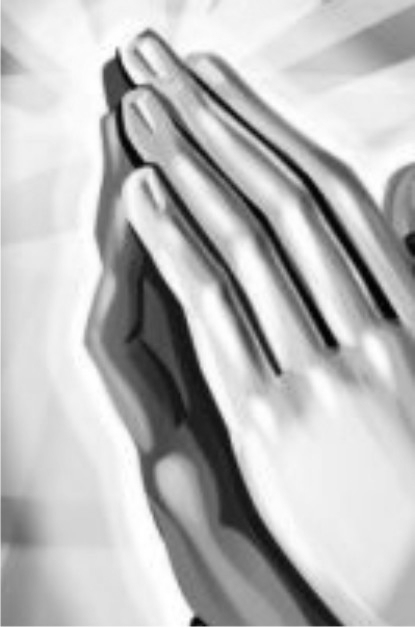
\includegraphics[scale=0.15]{gambar/bersyukur1.png}

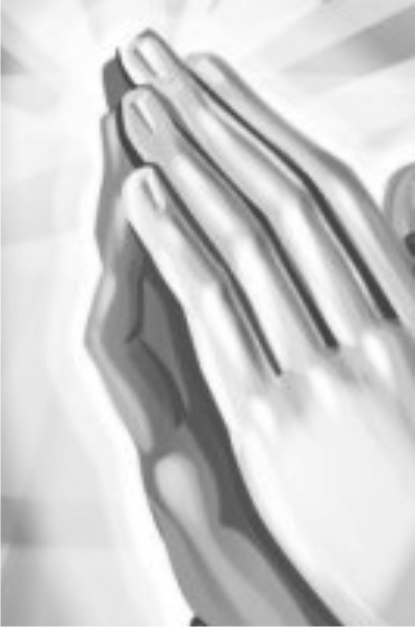
\includegraphics[scale=0.15]{gambar/bersyukur2.png}


\includegraphics[scale=0.15]{gambar/bersyukur3.png}


\includegraphics[scale=0.15]{gambar/bersyukur4.png}

\end{wrapfigure}

{~}

\begin{itemize}[label=\ding{62}]
\item Bersyukurlah bahwa kamu belum siap memiliki segala sesuatu yang kamu inginkan. Seandainya sudah, apalagi yang harus diinginkan?


\item Bersyukurlah apabila kamu tidak tahu sesuatu. Karena itu memberimu kesempatan untuk belajar.

\item Bersyukurlah untuk masa-masa sulit. Di masa itulah kamu tumbuh...

\item Bersyukurlah untuk keterbatasanmu. Karena itu memberimu kesempatan untuk berkembang.
\end{itemize}

\begin{itemize}[label=\ding{62}]
\item Bersyukurlah untuk setiap tantangan baru. Karena itu akan membangun kekuatan dan karaktermu.

\item Bersyukurlah untuk kesalahan yang kamu buat. Itu akan mengajarkan pelajaran yang berharga.

\item Bersyukurlah bila kamu lelah dan letih. Karena itu kamu telah membuat suatu perbedaan.

\item Mungkin mudah untuk kita bersyukur akan hal-hal baik...

\item Hidup yang berkelimpahan datang pada mereka yang juga bersyukur akan masa surut...

\item Rasa syukur dapat mengubah hal yang negatif menjadi positif ...

\item Temukan cara bersyukur akan masalah-masalahmu dan semua itu akan menjadi berkah bagimu ...
\end{itemize}

\sumber{Rahardi, Rian. ``Bersyukurlah.''\\  
www.renungan-harian-kita.blogspot.com.}

\newpage
\chap{Kompendium Katekese Gereja Katolik}
\setcounter{kgkcounter}{13}
{\normalsize

\kgk{Apa hubungan antara Tradisi dan Kitab Suci?}
    Tradisi dan Kitab Suci berhubungan erat dan saling melengkapi. Masing-           
masing menghadirkan misteri Kristus dan berbuah di dalam Gereja. Kedua hal ini       
mengalir dari satu sumber ilahi yang sama, dan bersama-sama membentuk khazanah
iman yang suci dan dari sinilah Gereja mendapatkan kepastian tentang wahyu.

\kgk{Kepada siapa iman ini dipercayakan?}
Para Rasul mempercayakan khazanah iman ini kepada seluruh Gereja.
Berkat makna iman yang adikodrati inilah umat Allah secara keseluruhan, dengan
bimbingan Roh Kudus dan dituntun oleh Kuasa Mengajar Gereja, tidak pernah
berhenti untuk menerima, meresapkan lebih dalam, dan menghayati anugerah
wahyu ilahi ini secara lebih penuh.

\kgk{Kepada siapa diberikan tugas untuk menafsirkan khazanah iman ini
secara autentik?}
Tugas untuk memberikan tafsir autentik terhadap khazanah iman ini diper-
cayakan kepada otoritas Kuasa Mengajar Gereja, yaitu pengganti Petrus, Uskup
Roma, dan para Uskup yang ada dalam kesatuan dengannya. Dalam pelayanan
Sabda Allah, pengajaran resmi ini mempunyai karisma kebenaran, dan kepadanya
juga diberi tugas untuk merumuskan dogma yang merupakan rumusan kebenaran
yang terdapat dalam wahyu Ilahi. Otoritas pengajaran resmi ini juga diperluas pada
kebenaran-kebenaran lain yang mempunyai hubungan erat dengan wahyu.

\kgk{Apa hubungan antara Kitab Suci, Tradisi, dan Kuasa Mengajar?}
Kitab Suci, Tradisi, dan Kuasa Mengajar berhubungan erat satu sama lain
sedemikian sehingga yang satu tidak dapat ada tanpa yang lain. Dengan bekerja
sama, masing-masing dengan caranya sendiri, ketiga hal tersebut memberikan
sumbangan secara efektif bagi keselamatan jiwa-jiwa di bawah naungan karya
Roh Kudus.

\flushright{(\dots \emph{bersambung} \dots)}
}
\end{document}